% !TeX spellcheck = en_US
\documentclass[a4paper,12pt]{article}


\usepackage[english]{babel}
\usepackage[T1]{fontenc}
\usepackage[toc,page]{appendix}
\usepackage{amssymb}
\usepackage{amsmath}
\usepackage{latexsym}
\usepackage{physics}
\usepackage[a4paper,left=0.7cm,right=0.7cm]{geometry}
\usepackage{wrapfig}
\usepackage{graphicx}
\usepackage{multicol}



\title{%
	Quantum Information \\
	\large Exercise 1 \\
}
\author{Vincenzo Maria Schimmenti - 1204565}

\begin{document}
\sloppy
	
	
\maketitle

\section*{Exercise 1.2}
In this exercise we had to sum in Fortran the integer numbers $2'000'000$ and $1$ and the real numbers $\pi \times 10^{32}$ and $\sqrt{2} \times 10^{21}$ using different types of number. For the integers we used the \textbf{integer*2} (2 bytes) and the \textbf{integer*4} (4 bytes); for the reals \textbf{real*4} and \textbf{real*8}.\\
Using \textbf{integer*2} (and the compiler flag \textit{-fno-range-check}) we get that the resulting integer is $-31615$ which in two's complement is $1000010010000001$; $2'000'000$ must be represented with more than $16$ bits as $0111101000010010000000$ so we encounter a truncation error: indeed the above unexpected number can be understood if we add one to $2'000'000$  and with take the first $16$ least significant bits. Everything works fine if we use \textbf{integer*4} since it has enough bits to store $2'000'000$ and the resulting addition with $1$. \\
In the \textbf{real*4} representation the values $\pi \times 10^{32}$ and $\sqrt{2} \times 10^{21}$ are represented as $3.14159278E+32$ and $1.41421360E+21$ and the summation is $3.14159278E+32$, i.e. we see no difference with the first addend, since the \textbf{real*4} has not enough precision and $\sqrt{2} \times 10^{21}$ exceeds it. The same does not happen with \textbf{real*8}: the numbers are represented as $3.1415926535897933E+032$ and $1.4142135623730950E+021$ and the resulting summation is $3.1415926536039354E+032$, hence we observe that the double precision is able to take into account the addition of $\sqrt{2} \times 10^{21}$.
\section*{Exercise 1.3}
In this exercise we measure the performance of matrix multiplication algorithm; we compare two coded algorithms and the Fortran intrinsic one. The two coded algorithms follow the naive matrix multiplication algorithm (which is $O(N^3)$): the only difference is that the second we implement is optimized for the allocation policy for matrices in Fortran, which is column-wise. Indeed every algorithm does a computation like:
\begin{equation*}
	c(i,j) <= c(i,j)+a(i,k) \times b(k,j)
\end{equation*}
where $<=$ stands for an assignment operator. The matrices $a$ and $b$ are the ones we want to multiply; $c$ is the resulting one. The three indices are \textit{borrowed} from the standard multiplication formula:
\begin{equation*}
	c_{ij} = \sum_{k=1}^N a_{ik} b_{kj}
\end{equation*}
The standard way of implementing the algorithm is by means of three for loops; the more intuitive method is the one starting with the $i$ loop, which is followed by $j$ and $k$. However this order (which we call \textit{method 1}) is efficient for matrix store row-wise so we need to reverse the order of the indices to get a good performance (from the cache point of view) on column-wise stored matrices, like in Fortran: indeed this way we first loop into $k$ then into $j$ and $i$ (this way the $k$ index runs slower being a column index increasing the performance). The third method we use is the most efficient one and is the one intrinsic of Fortran. Below we show the results. The first picture uses the standard compile command while the other three are compiled using, respectively, the optimization flags $-O1$, $-O2$, $-O3$ and $-O3 -Ofast$.\\
In general the performance of the intrinsic algorithm is way better than the other two; we can notice slightly better execution times for the cache optimized algorithm (method 2). Instead in our study case moving from the non-optimized code to any of the optimized ones we gain an order of magnitude of performance (i.e. we have an execution time on average ten times smaller).
\begin{figure}[h]
	\centering
	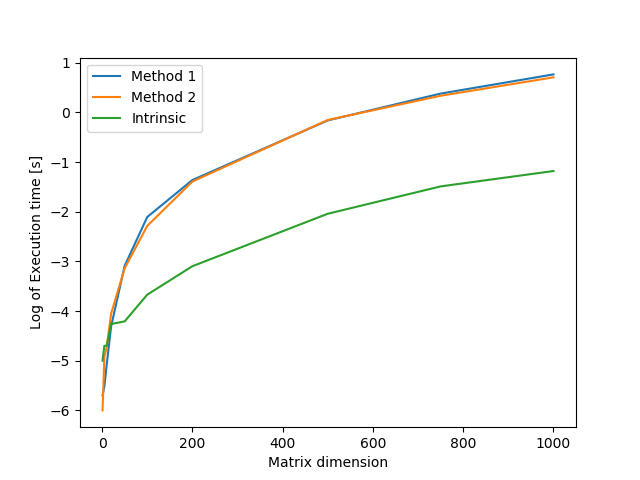
\includegraphics[width=0.6\textwidth]{perf.png}
	\caption{Log of execution time vs matrix dimension for matrix multiplication}
\end{figure}
\begin{figure}[h]
	\centering
	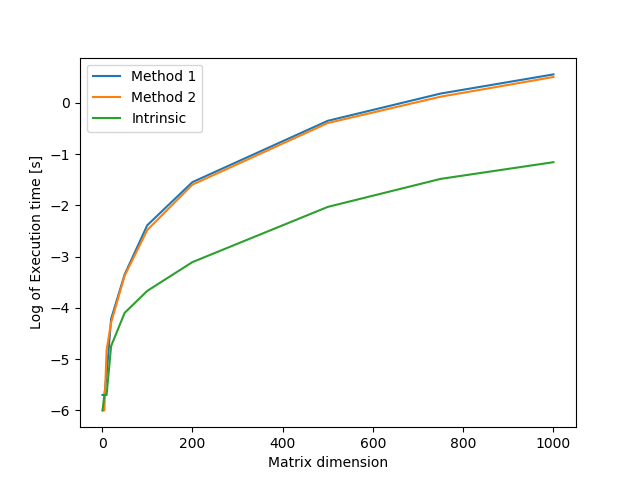
\includegraphics[width=0.6\textwidth]{perfO1.png}
	\caption{Log of execution time - Optimization O1}
\end{figure}
\begin{figure}[h]
	\centering
	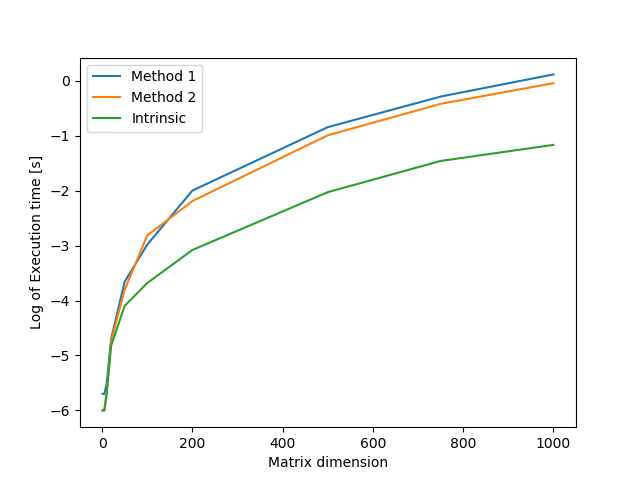
\includegraphics[width=0.6\textwidth]{perfO2.png}
	\caption{Log of execution time - Optimization O2}
\end{figure}
\begin{figure}[h]
	\centering
	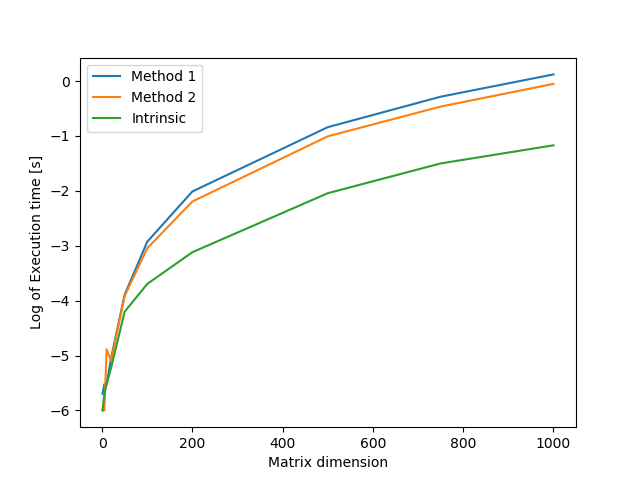
\includegraphics[width=0.6\textwidth]{perfO3.png}
	\caption{Log of execution time - Optimization O3}
\end{figure}
\begin{figure}[h]
	\centering
	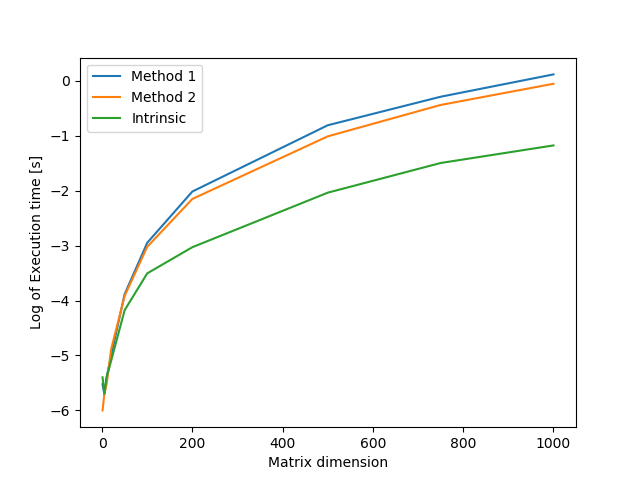
\includegraphics[width=0.6\textwidth]{perfO3fast.png}
	\caption{Log of execution time - Optimization O3 fast}
\end{figure}
\end{document}